%%%% Proceedings format for most of ACM conferences (with the exceptions listed below) and all ICPS volumes.
\documentclass[acmsmall]{acmart}
\usepackage{multirow}
\usepackage{listings}
\usepackage{subcaption}
\usepackage[T1]{fontenc}

\def\BibTeX{{\rm B\kern-.05em{\sc i\kern-.025em b}\kern-.08emT\kern-.1667em\lower.7ex\hbox{E}\kern-.125emX}}
\acmYear{2022} \acmVolume{1} \acmNumber{1} \acmArticle{1} \acmMonth{1}
\acmDOI{10.1145/3418301}
\acmISBN{123-4567-24-567/08/06}
\acmJournal{TOCE}
\acmYear{2022} \acmVolume{1} \acmNumber{1} \acmArticle{1} \acmMonth{1}
\copyrightyear{2022}
\acmPrice{15.00}

\begin{document}
\title[RadGrad: Results of a case study]{Improving engagement, diversity, and retention in computer science with RadGrad: Results of a case study}

\author{Philip M. Johnson}
\email{johnson@hawaii.edu}
\author{Carleton Moore}
\email{cmoore@hawaii.edu}
\affiliation{%
  \institution{Department of Information and Computer Sciences, University of Hawaii at Manoa}
  \city{Honolulu}
  \state{HI}
  \postcode{96822}
}

\author{Peter Leong}
\email{peterleo@hawaii.edu}
\author{Seungoh Paek}
\email{spaek@hawaii.edu}
\affiliation{%
  \institution{Department of Learning Design and Technology, University of Hawaii at Manoa}
  \city{Honolulu}
  \state{HI}
  \postcode{96822}
}
\orcid{0000-0002-9508-9225}

\renewcommand{\shortauthors}{Johnson et al.}

\newcommand{\AbstractCategory}[1]{%
  \par\addvspace{.5\baselineskip}% adjust to suit
  \noindent\textbf{#1}\quad\ignorespaces
}

\begin{abstract}

\AbstractCategory{Objectives}
RadGrad is a curriculum initiative implemented via an application that combines features of social networks, degree planners, individual learning plans, and serious games. RadGrad redefines traditional meanings of ``progress'' and ``success'' in the undergraduate computer science degree program in an attempt to improve engagement, retention, and diversity. In this paper, we describe the RadGrad Project and report on an evaluation study designed to assess the impact of RadGrad on student engagement, diversity, and retention. We also present opportunities and challenges that result from the use of the system.

\AbstractCategory{Participants}
Our evaluation study involved several major stakeholder groups for undergraduate computer science education at our institution, including: 498 students, 11 Faculty, and 2 Advisors.

\AbstractCategory{Study Methods}
We used a qualitative experimental research design, including data obtained through questionnaire responses from our major stakeholder group as well as data from system instrumentation.

\AbstractCategory{Findings}
We found strong evidence to support the hypothesis that RadGrad can have a positive impact on student engagement in Computer Science for students who are relatively new to the discipline. We found some evidence to support the hypothesis that RadGrad can have a positive impact on student diversity. We were unable to evaluate the impact of RadGrad on retention.

\AbstractCategory{Conclusions}
The data gathered in this study indicates that approaches like RadGrad provide a promising means to improve engagement, diversity, and (potentially) retention in Computer Science.  The data suggests that development and evaluation of RadGrad at other institutions and/or in other STEM disciplines would provide useful insight into the generality of the approach. It also indicates that faculty engagement with the technology would increase its effectiveness, but that obtaining faculty buy-in is challenging.

\end{abstract}

\begin{CCSXML}
<ccs2012>
<concept>
<concept_id>10003456.10003457.10003527.10003538</concept_id>
<concept_desc>Social and professional topics~Informal education</concept_desc>
<concept_significance>500</concept_significance>
</concept>
<concept>
<concept_id>10003456.10003457.10003527.10003539</concept_id>
<concept_desc>Social and professional topics~Computing literacy</concept_desc>
<concept_significance>500</concept_significance>
</concept>
</ccs2012>
\end{CCSXML}

\ccsdesc[500]{Social and professional topics~Informal education}
\ccsdesc[500]{Social and professional topics~Computing literacy}

\keywords{Curriculum Initiative; Diversity; Engagement; Retention}

\maketitle

\section{Introduction}

\subsection{Research Problem}
{\em\small Frame the problem or question and its context. Review, critique, and synthesize the applicable literature to identify key issues/debates/theoretical frameworks in the relevant literature to clarify barriers, knowledge gaps, or practical needs.}

Traditional curriculum initiatives for undergraduate computer science generally fall into one of three categories. The first involves the injection of a specific technology across the curriculum, such as initiatives for cloud computing \cite{deb_module-based_2019}. The second involves the injection of a specific domain across the curriculum, such as initiatives for cybersecurity \cite{tang_shaping_2019} or distributed computing \cite{abebe_watdfs:_2019}. The third involves the integration of practices intended to address demographic problems including lack of access or diversity, such as initiatives at the University of Illinois \cite{metcalf_diversity_2018} and University of Oklahoma \cite{collain_you_2019}.

One problem with these types of curriculum initiatives is that they all require changing, well, the curriculum.  This is a problem because changing the curriculum is hard: any significant curriculum change will require the approval of committees at multiple levels of the educational institution, it will require buy-in across the faculty, and it will often require significant resources to implement and sustain.

A benefit of changing the curriculum is that if it is accomplished, then {\em student} buy-in is normally not required. Because the change is to the curriculum, if a student wants to graduate, then they must follow the changed curriculum.

At our University, we have been experimenting with an initiative called "RadGrad", which falls outside these typical categories of curriculum initiatives, and as a result inverts the typical problems and benefits associated with traditional curriculum initiatives.

RadGrad originally rose from two insights: first, a recognition that our department did not have the resources to enable its undergraduate curriculum to keep up with the rate of change in computer science technology and the ever widening domain of application areas, nor could we keep up with student demand for access to curriculum content.  In some cases, the local high tech community or online educational services could fill in the gaps, but our department provided no support for student awareness of these extracurricular resources, or guidance as to which ones were worth spending time on, or how such activities might integrate with existing curricular offerings.  Finally, since extracurricular activities, are, by definition, "extra", there is a structural incentive for students to limit these activities and instead focus on curricular work which directly affects their GPA.

Second, we recognized that the increase in demand for our undergraduate computer science degree programs was paradoxically leading to a decrease in the diversity of our student body. Increasingly few women and underrepresented groups were making it all the way through our program to graduation. Although approximately 40\% of our first year students each year are women, only 15\% of our graduating seniors in AY 2018 were women.

In an attempt to address these issues, we created RadGrad, which is a web-based application that combines features of social networks, degree planners, and serious games.  Undergraduate students interested in our major can login to RadGrad and declare their interests and career goals. The system then recommends faculty-curated extracurricular opportunities matching their preferences. A degree planner tool enables students to lay out their "degree experience" as a combination of curricular activities (courses) and extracurricular activities (internships, meetups, online courses, hackathons, etc) for each upcoming semester until their planned graduation date. Finally, RadGrad enables students to learn about the broader ways in which computer science impacts upon local, national, and global society, as well as helping them to connect with and create communities of practice inside and outside of the department. As will be discussed below, related research suggests that making these connections can improve student engagement, diversity, and retention.

To combat the view of extracurricular activities being perceived as "extra", RadGrad does not use GPA to represent student success or progress. Instead, RadGrad provides a three component metric called "ICE", an acronym for Innovation, Competency, and Experience. Students are awarded Competency points for successfully completing a course, and a varying amount of Innovation and/or Experience points for successfully completing an extracurricular activity defined within the system. For example, participating in a hackathon will earn some number of Innovation points, since the goal of hackathons is to create something new.  Finishing a summer internship in a high tech company will earn Experience points since that activity provides students with a sense for the demands of a high tech workplace environment. (Depending upon the nature of the internship, it could also earn Innovation points.) To "win" at RadGrad, students must (among other things) earn at least 100 Innovation, Competency, and Experience points by completing some combination of curricular and extracurricular activities by the time they graduate.

Unlike traditional curriculum initiatives, RadGrad exists apart from the official curriculum requirements for our degree programs. As a result, we have been free to deploy and experiment with the approach without the multi-year approval process normally required for curriculum changes.  On the down-side, participation in RadGrad is voluntary, and so students must opt in to the system and its philosophy to gain its benefits.

\subsection{Research Goals}
{\em\small State the purpose(s)/goal(s)/aim(s) of the study. State the target audience, if specific. Provide the rationale for fit of design used to investigate this purpose/goal (e.g., theory building, explanatory, developing understanding, social action, description, highlighting social practices). Describe the approach to inquiry, if it illuminates the objectives and research rationale (e.g., descriptive, interpretive, feminist, psychoanalytic, postpositivist, critical, postmodern, constructivist, or pragmatic approaches).}

RadGrad began in the Fall of 2015 as a student-driven project in several upper-division software development courses.  A common perspective from students working on the project at that time was, "I wish I'd had RadGrad when I was starting out in Computer Science".  However, most of these students were high achieving, soon-to-graduate individuals who were demonstrating an ability to successfully finish a computer science degree program without the aid of RadGrad.  While we found their feedback to be encouraging, we wanted to know whether RadGrad would be interesting and/or useful to students who were more "at risk" in our program. Ideally, we wanted to know if the insights that RadGrad provides regarding the spectrum of computer science careers as well as extracurricular opportunities in the discipline both during and after the degree program would lead to a more diverse and engaged student body, with less attrition over the course of the degree program.

Unfortunately, there have been a multitude of impacts on our computer science degree program over the years of the RadGrad Project, ranging from curricular revisions to changes in advising personnel and process to the biggest impact of them all: COVID-19.  Our research approach cannot unambiguously separate the impact of RadGrad on engagement, retention, and diversity from all of these other factors.  While we will report on institutional data regarding diversity and retention, our approach focuses on qualitative perspectives from a variety of stakeholders (students, faculty, and advisors) on their view of RadGrad and the use of this data to assess the potential of RadGrad to impact engagement, diversity, and retention, along with insights into how to improve the project in the future.

More specifically, during Academic Year 2021-2022, we conducted a qualitative case study that was designed to provide evidence regarding the following research questions:

\begin{itemize}
\item Do students, when introduced to RadGrad, find it of value to their educational experience?
\item Do students, after completing their degree program, view RadGrad as having improved their educational experience?
\item What are the views of Faculty and Advising staff regarding RadGrad/
\item What do these findings imply regarding engagement, diversity, and retention in computer science undergraduate degree programs?
\end{itemize}

We report on this study starting in Section \ref{sec:method}. First, however, we step back to better motivate the design of RadGrad, as well as describe the system in more detail.

\section{Related Work}
\label{sec:related-work}

There is a national need for undergraduate computer science degree programs to improve both retention (the percentage of students entering CS programs who finish the degree) and diversity (the percentage of graduates who are female and/or from an underrepresented minority group).  We need to improve retention because the projected demand for skills in computer science far exceeds current production \cite{camp_generation_2017}.  We need to improve diversity because a more diverse STEM population improves tech innovation at large. For example, mixed-sex teams filed 40\% more information and technology patents than all-male teams \cite{ashcraft_who_2012}, and management diversity leads to a \$42M increase in S\&P value of firms \cite{dezso_girl_2007}.

While the need is clear, solutions are complicated. Gender diversity in computer science has actually fallen in the last 20 years \cite{hong_women_2014}, with no well accepted explanation for its cause. Some diversity-related issues start in middle and high school: black students are less likely than white students to have computer science courses in middle and high school, and female students are less likely than male students to be told they would be good at computer science \cite{inc_diversity_2016}.   There is some research that provides evidence for a way forward: a study by Google \cite{hong_women_2014} concludes that four factors primarily influence young womens' decision to pursue CS: (1) social encouragement (positive reinforcement of CS pursuits from family and peers); (2) self perception (an interest in problem solving and a belief that those skills can be translated to a successful career); (3) academic exposure (availability of curricular and extracurricular CS activities); and (4) career perception (view of CS as a career with diverse applications and a broad potential for positive societal impact). Stout and Camp \cite{stout_now_2014} make similar points around social relevance, a sense of belonging, and cultural bias. RadGrad implements capabilities designed to help address isssues around self perception, academic exposure, career perception, and social relevance among its student users.

For those high school students who graduate and enter an undergraduate degree program in computer science, retention becomes a significant issue.   More than half of the students who start out in science or engineering switch to other majors or do not finish college at all \cite{kober_reaching_2015}. Initiatives to improve retention, such as the Threads undergraduate curriculum at Georgia Tech, emphasize giving students more control over their degree plan, a better understanding of how their studies relate to their career interests, and an increased emphasis on the importance of extracurricular activities \cite{barrett_expanding_2017}. RadGrad provides a technology platform, information system, and incentive structure with these emphases.

Communities of Practice (CoP) is a theory of learning first proposed in 1991 \cite{lave_situated_1991}, more fully developed in 1998 \cite{wenger_communities_1998}, and extended to "landscapes of practice" in 2004 \cite{wenger_learning_2004}. A loose definition of Communities of Practice is "groups of people who share a concern or a passion for something they do and learn how to do it better as they interact regularly." More specifically, three characteristics distinguish a community of practice from other kinds of communities: (1) There is at least one domain of interest shared by all members; (2) members engage in joint activities and discussions, help each other, and share information;  and (3) members are practitioners in the domain, not just people with shared interests, and thus develop a shared repertoire of resources.

Communities of Practice show great promise for improving undergraduate retention and diversity, because participating students will find a new source for social encouragement, self-perception, academic exposure, and career perception. In undergraduate degree programs, CoPs are primarily found within disciplinary-specific extracurricular activities: clubs, meetups, hackathons, and so forth. RadGrad makes these CoPs visible to students, and provides incentives to students for participating in them.

\section{RadGrad}
\label{sec:radgrad}

The RadGrad project began in the Fall of 2015. For the first few years, development was student-led as part of various software engineering classes. Development activities during this time focused on the underlying data model, user interface mockups, and possible game mechanics. In 2017, a pilot implementation was deployed into a computer science department and some we began receiving user feedback. In 2018, we began work on RadGrad Version 2, an "industrial strength" version of the system that followed high quality software engineering practices and would enable deployment to different institutions and disciplines. RadGrad is now a fully functional web-based application, implemented in approximately 30,000 lines of Javascript and 7,000 lines of HTML. It has extensive design and development documentation, unit and integration tests, and implements continuous integration. Instances can be deployed locally or using a cloud-based hosting service such as Digital Ocean. Over 1,000 students have used RadGrad to date.

Figure \ref{fig:radgrad} shows the RadGrad Degree Plan page which illustrates several capabilities of the system. The left side contains a four by three grid representing four academic years each containing three semesters (Fall, Spring, Summer).  For each of the 12 semesters, this hypothetical student indicates not just their CS-related curricular activities (i.e. Courses) but also their CS-related extracurricular activites (called "Opportunities" in RadGrad).

\begin{figure}[ht]
\centering
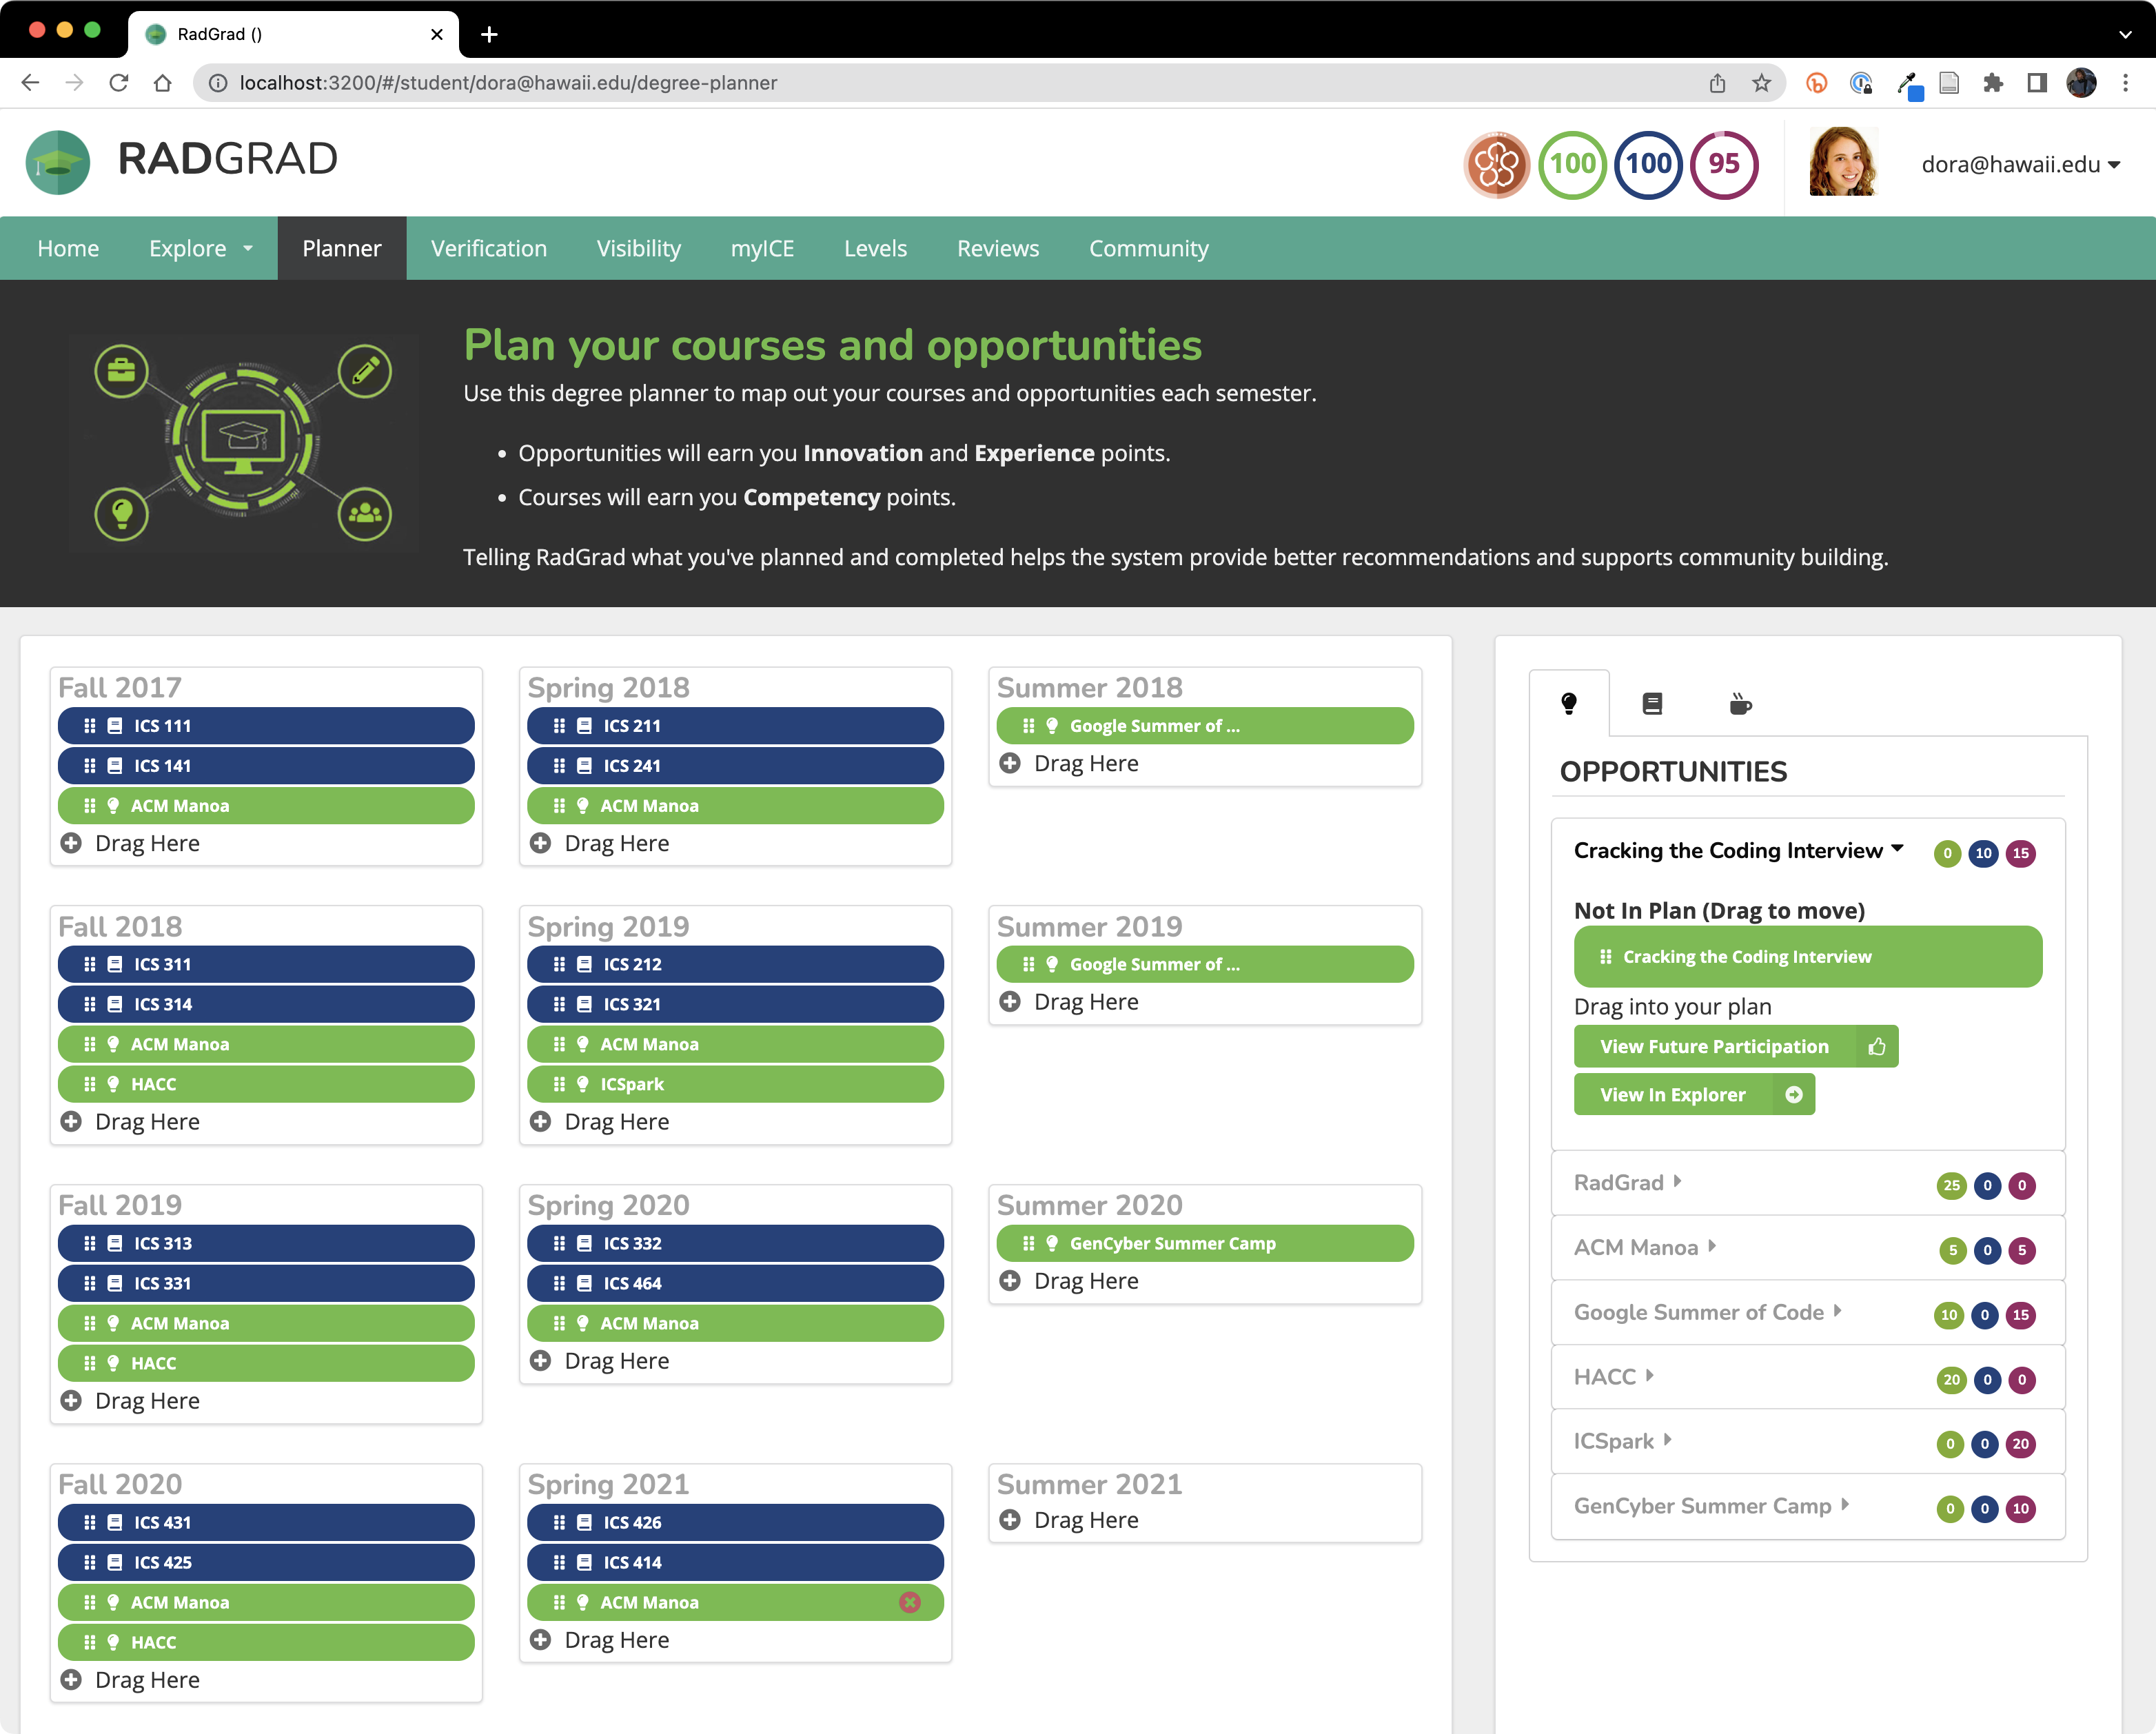
\includegraphics[width=\linewidth]{dora-planner.eps}
\caption{\em RadGrad Degree Plan page}
\label{fig:radgrad}
\end{figure}

The right hand side has two panes, one providing an "Inspector" and one providing an "Academic Plan" browser. The Inspector allows students to browse the currently available Courses and Opportunities and learn details about them including a description, links to external resources, the number of ICE points that can be earned by completing the Course or Opportunity, and which (if any) of the student's declared Interests are matched by the Course or Opportunity. The Academic Plan browser presents the set of academic plans available to that student (i.e. "B.S. Computer Science", "B.A. Computer Science", etc.) along with a canonical 8 semester plan to complete the coursework for the degree. The Academic Plan shows a course in green if it is present in the student's plan, and red if it not yet added. A drag-and-drop UI allows students to easily take Courses from the Academic Plan pane and put them into their Degree Plan.

Each page has a documentation pane that is displayed with a light green background and is located just below the navbar. Clicking the triangle on the left side reveals documentation about the current page.

For students, the RadGrad UI is organized into four top-level pages as shown in the tabbed area underneath the navbar.  The Home page provides a place for students to update their profile to indicate their current Career Goals and Interests, as well as personal information such as their picture and personal home page.  The Explorer page allows students to browse Courses, Opportunities, Career Goals, Interests, and Academic Plans.  The Degree Planner page (as show in Figure \ref{fig:radgrad}) allows students to design their degree experience as a combination of curricular and extracurricular activities.  The Mentor Space page provides a mechanism for students to engage with alumni and local high tech professionals to learn more about career opportunities and other information about professional life.

Figure \ref{fig:ice} zooms in on the portion of the navigation bar containing a student's Level ( a green RadGrad icon) and ICE Points (three circles containing numbers inside). RadGrad provides a game mechanic consisting of six "Levels", each represented by a different colored RadGrad icon. As students earn ICE Points and carry out other RadGrad activities, such as writing reviews of courses and opportunities, they can progress through white, yellow, green, blue, brown, and black levels, similar to martial art belt colors. The rules for achieving Levels are designed such that a motivated student can achieve a new Level each semester, so a total of six semesters (typically three years) is required to get through all Levels. We print laptop stickers for each Level, and students can get a new laptop sticker free from the department with the color corresponding to each Level as they achieve it. This provides visibility for RadGrad and for the student's participation.  The student in Figure \ref{fig:ice} is currently at Level 3 (green).

\begin{figure}[h]
\centering

\includegraphics[width=\linewidth]{ice-points-navbar.png.eps}
\caption{\em UI for student Level and ICE Points}
\label{fig:ice}
\end{figure}

We developed a circular representation for ICE Points to help students quickly understand their progress using RadGrad.  Achieving a successful undergraduate degree experience according to RadGrad's game mechanics means that a student must first plan out a sequence of curricular and extracurricular activities that will eventually earn them at least 100 Innovation, Competency, and Experience points. Once they have made that plan (which they are free to change at any time), they must then actually earn the points by completing the curricular and extracurricular activities. To verify completion of a curricular activity, RadGrad imports data from the University's course management system indicating the coursework the student has taken and the grade they received.  To verify completion of an extracurricular activity, the student must first "request verification" of the Opportunity.  This request sends a message to the RadGrad administrator or faculty member who has responsibility for checking that the student participated. The admin or faculty member can accept or decline the verification request, and if accepted, the system will award the points associated with the Opportunity to the student.

RadGrad represents ICE by three circles: a green circle for Innovation, a blue circle for Competency, and a red circle for Experience. For each of the three components of ICE, the circle is partially or fully colored in a light shade to represent the number of {\em planned} points, based upon what the student has put in their degree plan. In Figure \ref{fig:ice}, the Innovation circle is colored only half way in a light green color, which indicates that this student has only planned to earn 50 Innovation points so far.  The blue circle is completely filled in, indicating that the student has planned to achieve 100 Competency points.  Finally, the Experience circle is also only half filled, indicating that only 50 Experience points are currently in the degree plan.

RadGrad uses a dark shade on the circle to represent the number of points actually earned so far, and also indicates that number in the center of the circle. So, the student in Figure \ref{fig:ice} has so far earned 5 Innovation, 78 Competency, and 5 Experience points.

Finally, RadGrad defines four other roles for users in addition to Student: Admin, Faculty, Advisor, and Mentor. The user interface to RadGrad varies significantly in functionality depending upon the role of the user.  For example, users with the Advisor role have the ability to add new students to the system, and see existing student degree plans. Due to space limitations, only a brief overview of functions and capabilities associated with the Student role are described in this section. For more detailed information about the system, please go to https://radgrad.org.




\section{Method}
\label{sec:method}

\subsection{Research Design Overview}

{\em\small  Summarize the research design, including data-collection strategies, data-analytic strategies, and, if illuminating, approaches to inquiry (e.g., descriptive, interpretive, feminist, psychoanalytic, postpositivist, critical, postmodern, constructivist, or pragmatic approaches). Provide the rationale for the design selected.}

\subsection{Study Participants}

\subsubsection{Researcher Description}

{\em\small Describe the researchers’ backgrounds in approaching the study, emphasizing their prior understandings of the phenomena under study (e.g., interviewers, analysts, or research team). Describe how prior understandings of the phenomena under study were managed and/or influenced the research (e.g., enhancing, limiting, or structuring data collection and analysis).}

\subsubsection{Participants}

{\em\small Provide the numbers of participants/documents/events analyzed. Describe the demographics/cultural information, perspectives of participants, or characteristics of data sources that might influence the data collected. Describe existing data sources, if relevant (e.g., newspapers, internet, archive). Provide data repository information for openly shared data, if applicable. Describe archival searches or process of locating data for analyses, if applicable. }


\subsubsection{Researcher–Participant Relationship}

{\em\small  Describe the relationships and interactions between researchers and participants relevant to the research process and any impact on the research process (e.g., was there a relationship prior to research, are there any ethical considerations relevant to prior relationships). }


\subsection{Participant Recruitment}
\subsubsection{Recruitment Process}

{\em\small Describe the recruitment process (e.g., face-to-face, telephone, mail, email) and any recruitment protocols. Describe any incentives or compensation, and provide assurance of relevant ethical processes of data collection and consent process as relevant (may include institutional review board approval, particular adaptations for vulnerable populations, safety monitoring). Describe the process by which the number of participants was determined in relation to the
study design. Provide any changes in numbers through attrition and final number of participants/sources (if relevant, refusal rates or reasons for dropout). Describe the rationale for decision to halt data collection (e.g., saturation). Convey the study purpose as portrayed to participants, if different from the purpose stated. }

\subsubsection{Participant Selection}

{\em\small Describe the participants/data source selection process (e.g., purposive sampling methods, such as maximum variation; convenience sampling methods, such as snowball selection; theoretical sampling; diversity sampling) and inclusion/exclusion criteria. Provide the general context for the study (when data were collected, sites of data collection). If your participant selection is from an archived data set, describe the recruitment and selection process from that data set as well as any decisions in selecting sets of participants from that data set. }

\subsection{Data Collection}

\subsubsection{Data Collection/Identification Procedures}

{\em\small State the form of data collected (e.g., interviews, questionnaires, media, observation). Describe the origins or evolution of the data-collection protocol. Describe any alterations of data-collection strategy in response to the evolving findings or the study rationale. Describe the data-selection or data-collection process (e.g., were others present when data were collected, number of times data were collected, duration of collection, context). Convey the extensiveness of engagement (e.g., depth of engagement, time intensiveness of data collection). For interview and written studies, indicate the mean and range of the time duration in the data-collection process (e.g., interviews were held for 75 to 110 min, with an average interview time of 90 min). Describe the management or use of reflexivity in the data-collection process, as it
illuminates the study. Describe questions asked in data collection: content of central questions, form of questions (e.g., open vs. closed). }

\subsubsection{Recording and Data Transformation}

{\em\small Identify data audio/visual recording methods, field notes, or transcription processes used.}

\subsection{Analysis}

\subsubsection{Data-Analytic Strategies}

{\em\small Describe the methods and procedures used and for what purpose/goal. Explicate in detail the process of analysis, including some discussion of the procedures (e.g., coding, thematic analysis) following a principle of transparency. Describe coders or analysts and their training, if not already described in the researcher
description section (e.g., coder selection, collaboration groups). Identify whether coding categories emerged from the analyses or were developed a priori. Identify units of analysis (e.g., entire transcript, unit, text) and how units were formed, if applicable. Describe the process of arriving at an analytic scheme, if applicable (e.g., if one was
developed before or during the analysis or was emergent throughout). Provide illustrations and descriptions of the analytic scheme development, if relevant. Indicate software, if used. }

\subsubsection{Methodological Integrity}

{\em\small Demonstrate that the claims made from the analysis are warranted and have produced findings with methodological integrity. The procedures that support methodological integrity (i.e., fidelity and utility) typically are described across the relevant sections of a paper, but they could be addressed in a separate section when elaboration or emphasis would be helpful. Issues of methodological integrity include the following: Assess the adequacy of the data in terms of its ability to capture forms of diversity most relevant to the question, research goals, and inquiry approach. Describe how the researchers’ perspectives were managed in both the data collection and analysis (e.g., to limit their effect on the data collection, to structure the analysis). Demonstrate that findings are grounded in the evidence (e.g., using quotes, excerpts, or descriptions of researchers’ engagement in data collection). Demonstrate that the contributions are insightful and meaningful (e.g., in relation to the current literature and the study goal). Provide relevant contextual information for findings (e.g., setting of study, information about participants, interview question asked is presented before excerpt as needed). Present findings in a coherent manner that makes sense of contradictions or disconfirming evidence in the data (e.g., reconcile discrepancies, describe why a conflict might exist in the findings). Demonstrate consistency with regard to the analytic processes (e.g., analysts may use demonstrations of analyses to support consistency, describe their development of a stable perspective, interrater reliability, consensus) or describe responses to inconsistencies, as relevant (e.g., coders switching midway through analysis, an interruption in the analytic process). If alterations in methodological integrity were made for ethical reasons, explicate those reasons and the adjustments made. Describe how support for claims was supplemented by any checks added to the qualitative analysis. Examples of supplemental checks that can strengthen the research may include: transcripts/data collected returned to participants for feedback triangulation across multiple sources of information, findings, or investigators; checks on the interview thoroughness or interviewer demands; consensus or auditing process; member checks or participant feedback on findings; data displays/matrices; in-depth thick description, case examples, or illustrations; structured methods of researcher reflexivity (e.g., sending memos, field notes, diary, logbooks, journals, bracketing); checks on the utility of findings in responding to the study problem (e.g., an evaluation of whether a solution worked) }

\section{Findings}

{\em\small Describe research findings (e.g., themes, categories, narratives) and the meaning and understandings that the researcher has derived from the data analysis. Present research findings in a way that is compatible with the study design. Demonstrate the analytic process of reaching findings (e.g., quotes, excerpts of data). Present synthesizing illustrations (e.g., diagrams, tables, models), if useful in organizing and conveying findings. Photographs or links to videos can be used. }

\section{Discussion}

\subsection{Central Contributions to the Discipline}

{\em\small Describe the central contributions and their significance in advancing disciplinary understandings.}

\subsection{Types of Contributions Made by Findings}

{\em\small Describe the types of contributions made by findings (e.g., challenging, elaborating on, and supporting prior research or theory in the literature describing the relevance) and how findings can be best utilized. }

\subsection{Comparing Prior Theories and Research Findings}

{\em\small Identify similarities and differences from prior theories and research findings.}

\subsection{Alternative Explanations of Findings}

{\em\small Reflect on any alternative explanations of the findings.}

\subsection{Strengths and Limitations}

{\em\small Identify the study’s strengths and limitations (e.g., consider how the quality, source, or types of the data or the analytic processes might support or weaken its methodological integrity).}

\subsection{Limitations on Transferability}

{\em\small Describe the limits of the scope of transferability (e.g., what should readers bear in mind when using findings across contexts). }

\subsection{Ethical Dilemmas/Challenges}

{\em\small Revisit any ethical dilemmas or challenges that were encountered, and provide related suggestions for future researchers. }

\subsection{Implications for Future}

{\em\small Consider the implications for future research, policy, or practice.}

CS Education for the Socially-Just worlds we need

Confronting inequities: a case for critical theory

intersectional experiences of black women in computing

\section{Acknowledgements}

{\em\small Acknowledgments are placed before the references. Add information about grants, awards, or other types of funding that you have received to support your research. This information must be anonymized in the version of the paper you submit for review. }

\bibliographystyle{ACM-Reference-Format}
\bibliography{radgrad}



\end{document}
